\ylDisplay{Elektriskeem} % Ülesande nimi
{Tundmatu autor} % Autor
{lõppvoor} % Voor
{2014} % Aasta
{P 8} % Ülesande nr.
{2} % Raskustase
{
% Teema: Elektriõpetus

\ifStatement
Mitu korda erineb süsteemi maksimaalne ja minimaalne takistus sõltuvalt lülitite asendist? Esimene lüliti saab olla kas asendis $A$ või $B$ ning teine lüliti asendites $C$ või $D$ Kõikide takistite väärtused on $R = 1$ $\Omega$.
\begin{center}
	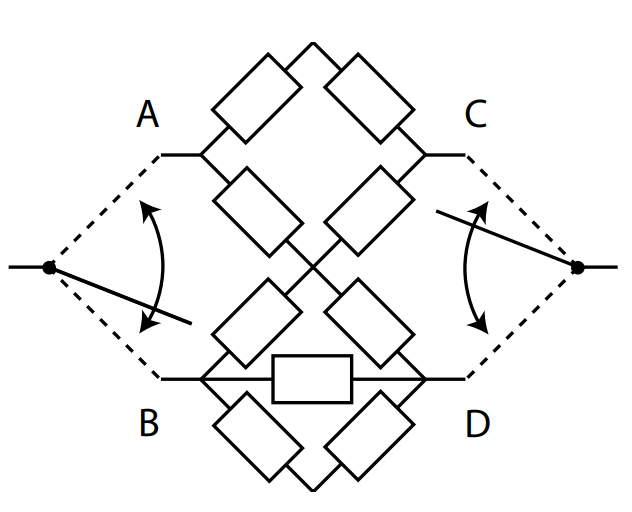
\includegraphics[width=0.5\linewidth]{2014-v3p-08-yl.png}
\end{center}
\fi

\ifHint
Ülesande lahendamisel aitab, kui skeem joonistada ümber lihtsamate jada- ja rööpühendustest koosneva segaühendusena.
\fi

\ifSolution
\begin{center}
	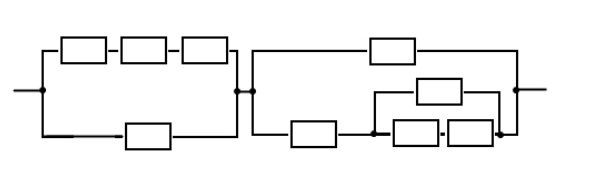
\includegraphics[width=0.5\linewidth]{2014-v3p-08-lah.png}
\end{center}
Asendites $AC$ (Esimene lüliti asendis $A$ ning teine asendis $C$) on süsteemi takistus $R$. Asendites $BD$ on süsteemi takistus $0,5$ $R$. Asendid $AD$ ning $BC$ on samaväärsed (vt joonis) omades kogutakistust $1 \frac{3}{8} R$ Seega erineb süsteemi maksimaalne ja minimaalne takistus $\frac{1 \cfrac{3}{8}R}{0,5R} = 2,75$ $korda$.
\fi
}
